\section{The frozen MSH evaluation}
\label{sec:msh}
\FloatBarrier

Every result reported so far comes from public sets, and every modeling
decision in this paper was made against the three development sets alone.
While the preceding sections were being written, Marvel Super Heroes
(MSH) had no public pick data at all: the set had not yet been drafted on
Arena when the evaluation protocol froze. This section reports what
happened when that data appeared.

\paragraph{The freeze.}
The protocol, its metric implementations, and the battery manifest are
fixed at the public git tag \texttt{\ProtocolTag}
(\S\ref{sec:protocol}). Each battery member's weights are anchored by a
sha256 hash committed to the experiment ledger before the test snapshot
existed, so the git history itself timestamps the claim that no model
saw MSH. The first public \seventeenlands{} MSH file was frozen at
download by its sha256 and ETag and never re-downloaded. There is one
evaluation round; running a second would require a new public tag and a
disclosure that a second round happened.

\paragraph{The single pass.}
One inference pass per battery member over the frozen snapshot produced
cached per-pick prediction files, and every MSH statistic in this paper
is computed from those files; no model has been re-run on MSH since.
The headline: F-full agrees with high-win-rate players' picks on
\FfullMsh\% of MSH picks, top-1, deployment mode (confidence interval in
Table~\ref{tab:main}). The pre-registered interpretation below was
drafted before that number existed and selected by it
(\S\ref{sec:protocol}).

% ======================================================================
% CLAIMS BAND ALTERNATIVES (pre-registered; docs/eval_protocol.md §6).
% Exactly ONE of the three paragraphs below is uncommented at MSH time,
% chosen solely by the frozen headline number. The text is drafted before
% the result exists and must not be softened or sharpened after the fact.
% Boundaries are set to the exact cited priors (44.54%, 55.44%), not
% rounded to 45%/55%, so no headline number can fall into a dead zone
% where the selected band's own cited-number claim would be false --
% fixed pre-T0, 2026-07-07, per Brian's explicit live decision (see
% docs/adversarial_review_2026-07-06.md and /tmp/DISCUSSION.md for the
% finding and the authorization to touch this frozen block this one time).
% ----------------------------------------------------------------------
% BAND A (< 44.54%):
% \paragraph{Interpretation.}
% The headline number falls short of the strongest day-one-feasible prior,
% the expert-tuned rating systems at 44.54\%: at current scale, multi-set
% training on public card features alone does not buy day-one competence,
% and hand-tuned expert ratings remain unbeaten at hour zero. The result is
% negative for the scaling hypothesis but leaves the contributions that do
% not depend on the headline: the frozen, tamper-evident benchmark; the
% first features-only multi-set zero-shot measurement; and the scaling
% curve, whose shape (Figure~\ref{fig:scaling}) indicates whether the gap
% is a data problem or a representation problem.
% ----------------------------------------------------------------------
% BAND B (44.54--55.44%):
% \paragraph{Interpretation.}
% The headline number makes DraftFM the strongest published day-one-feasible
% drafter we could locate: above expert-tuned ratings (44.5\%) and GPT-4o
% (43\%) -- each measured on a different test set than DraftFM's, so these
% situate rather than compare head-to-head -- and above every hour-zero
% heuristic we measure head-to-head on MSH itself. It remains below the
% 55.44\% of \citet{bertram2024cards} on
% held-out BRO. That number is the appropriate upper reference, and it is
% not a day-one number: its representation includes usage statistics
% computed from human play after release, information that by construction
% cannot exist when a set goes live. Within the information regime a
% deployed day-one assistant actually inhabits, DraftFM sets the published
% state of the art.
% ----------------------------------------------------------------------
% BAND C (> 55.44%): SELECTED -- frozen headline 57.01% > 55.44%, verified
% against scripts/run_frozen_eval.py output (frozen_eval/013df16b8994.../
% summary.json, executed 2026-07-07T23:59:34), 2026-07-08.
\paragraph{Interpretation.}
The headline number exceeds the strongest published unseen-set result,
the 55.44\% of \citet{bertram2024cards}, while using strictly less
information (no post-release usage statistics, no card images) on a
licensed-IP set with out-of-universe flavor (card names are masked
before embedding, \S\ref{sec:features}) -- a shift the dev-trio evidence
suggests text-masking mitigates but does not eliminate
(\S\ref{sec:analysis}). The BRO development row provides the
same-holdout anchor against that prior. Zero-shot drafting of an unseen
set is, on this evidence, better served by scale over public card
features than by any published use of post-release data.
% ======================================================================

\paragraph{The baselines did not survive the trip.}
The same pass scored the pre-registered hour-zero baselines on MSH, and
the result sharpens the day-one story. Random picking scores
\BaseRandomMsh\%, in line with its \BaseRandom\% pre-freeze rehearsal on
Secrets of Strixhaven. The rarity-and-color heuristic, which had reached
\BaseRarity\% on that rehearsal, collapses to \BaseRarityMsh\% on MSH:
barely above random (Table~\ref{tab:baselines}). Whatever surface
regularity the heuristic exploited on an in-universe development set did
not transfer to the licensed set, while the learned model held its
level. The gap between DraftFM and the best hour-zero alternative is
therefore widest exactly where day-one help matters.

\paragraph{Secondary detail from the same pass.}
The cached prediction file carries the pre-registered secondary
statistics as well. Top-3 agreement is \FfullMshTopThree\%, and mean
log-loss is \FfullMshLogLoss{} nats. Top-label ECE, at the temperature
fitted on the development trio and frozen before the snapshot existed
(\S\ref{sec:analysis}), is \FfullMshEce{}: tighter than any of the three
dev-trio figures rather than between them. We do not have a confirmed
explanation for that on this evidence. It is not simply forced picks
inflating the count of trivially well-calibrated predictions, since
MSH's non-forced ECE is close to its forced-inclusive figure, so we
report it without over-interpreting it. Scored on every valid pick
rather than the high-win-rate slice alone, agreement is
\FfullMshAllUsers\%, close to the headline. Finally, conditioning on
each drafter's own skill bucket instead of the fixed deployment bucket
leaves the high-win-rate number essentially unchanged (a
\FfullMshSkillGap{}pp difference), so the choice of conditioning bucket
matters as little on MSH as it does on the dev trio
(\S\ref{sec:analysis}).

\begin{table}[t]
  \centering
  \caption{Top-1 agreement (\%) by drafter win-rate band (bottom below
  0.50, middle 0.50--0.55, top 0.55 and above), deployment mode, on the
  three development sets and MSH, all computed from cached predictions.}
  \label{tab:skill-bands}
  \small
  % AUTO-GENERATED by scripts/make_paper_tables.py -- do not edit.
% Top-1 by drafter win-rate band, deployment mode, from cached predictions (eval_pick_breakdowns.py).
\begin{tabular}{lcccc}
\toprule
\rowcolor{tblhead}
Drafter band & BRO & TMT & SOS & MSH \\
\midrule
Bottom (win rate $<$ 0.50) & 47.8 {\scriptsize(47.6, 47.9)} & 57.4 {\scriptsize(57.1, 57.6)} & 56.6 {\scriptsize(56.5, 56.7)} & 56.4 {\scriptsize(56.2, 56.5)} \\  % run=20260704_135822_f_dev; run=20260704_135822_f_dev; run=20260704_135822_f_dev; run=frozen_eval/013df16b8994
Middle (0.50--0.55) & 48.4 {\scriptsize(48.3, 48.5)} & 58.1 {\scriptsize(57.9, 58.3)} & 57.0 {\scriptsize(56.9, 57.1)} & 56.9 {\scriptsize(56.7, 57.1)} \\  % run=20260704_135822_f_dev; run=20260704_135822_f_dev; run=20260704_135822_f_dev; run=frozen_eval/013df16b8994
Top ($\geq$ 0.55) & 48.8 {\scriptsize(48.7, 48.9)} & 57.8 {\scriptsize(57.7, 58.0)} & 56.8 {\scriptsize(56.7, 56.9)} & 57.1 {\scriptsize(56.9, 57.2)} \\  % run=20260704_135822_f_dev; run=20260704_135822_f_dev; run=20260704_135822_f_dev; run=frozen_eval/013df16b8994
\bottomrule
\end{tabular}

\end{table}

\paragraph{Who the model matches.}
Table~\ref{tab:skill-bands} breaks agreement out by drafter win-rate
band, using the same cached predictions. The striking feature is how
little the bands differ. On MSH the model agrees with the bottom band on
\SkillBandBotMsh\% of picks, the middle band on \SkillBandMidMsh\%, and
the top band on \SkillBandTopMsh\%, a spread of \SkillBandGapMsh{}pp
that rises mildly with drafter skill; under human-mode conditioning the
top and bottom bands sit at \SkillBandTopMshHuman\% and
\SkillBandBotMshHuman\%. The dev sets in the same table show the same
picture, with every band within about a point of its neighbors. The
model conditioned to imitate strong drafters agrees slightly more with
strong drafters, and it is not disproportionately reproducing weak
players' mistakes, but drafter skill moves agreement far less than which
set is being drafted does.

\begin{figure}[t]
  \centering
  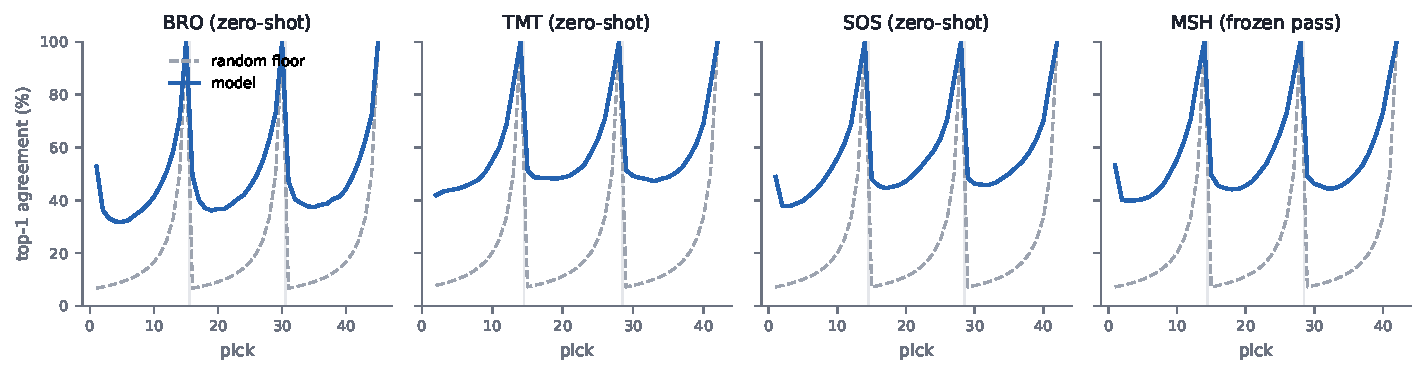
\includegraphics[width=\linewidth]{figures/pick_curves.pdf}
  \caption{Top-1 agreement with high-win-rate players at each pick
  position, against the per-cell random floor, on the three development
  sets and MSH. Forced final picks are trivially correct, which produces
  the end-of-pack spikes.}
  \label{fig:pick-curves}
\end{figure}

\paragraph{Accuracy through the draft.}
Figure~\ref{fig:pick-curves} plots top-1 agreement at every pick
position against the per-cell random floor, for the three development
sets and for MSH, all from the cached predictions. The margin over the
floor is the quantity to read, since later packs are smaller and forced
final picks are trivially correct. The dev-side question of
\S\ref{sec:analysis}, whether a set-agnostic model collapses toward
rate-the-card once pool context dominates, can be read off the MSH panel
the same way it was read off the trio.

\paragraph{What remains open.}
Two pre-registered post-day-one rows, a per-set ceiling trained on the
frozen MSH snapshot and F-full fine-tuned on MSH's own picks, are
deliberately not yet run, so the normalized score and late-draft
retention on MSH remain open for a follow-up release
(\pending{MSH per-set ceiling: normalized score and late-draft
retention}).
